\begin{practice}[sidebyside]{Traveling Salesmen}
\begin{center}
    \begin{tikzpicture}[
        every node/.style={
            secondaryaccent,
            fill=white,
            fill opacity=0.65,
            font=\bfseries\footnotesize,
            line width=2,sloped
        },every edge/.style={draw,edges,tertiaryaccent},
        scale=0.95,transform shape
    ]
    % Map
        \node[opacity=0.45] at (0,0) {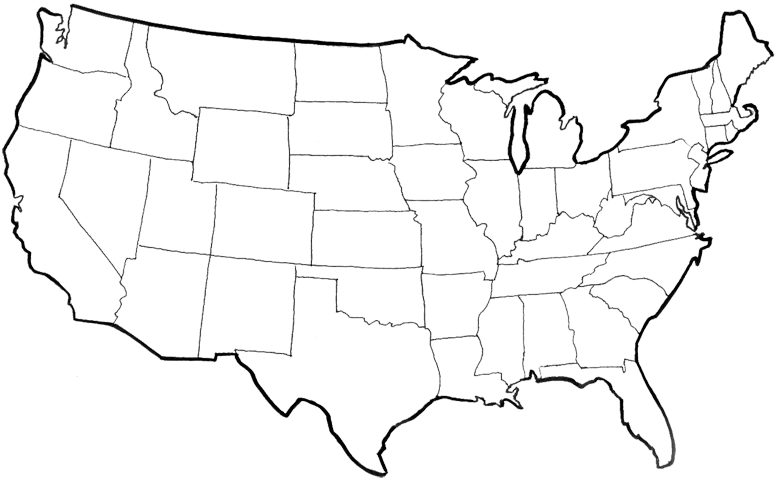
\includegraphics[width=\textwidth]{images/USA-Map-Transparent-Free-PNG-Clip-Art.png}};
    % Vertices
        \node[vertex] (S) at (-3.25,2.25) {S};
        \node[vertex] (L) at (-3.5,-0.5) {L};
        \node[vertex] (C) at (1.3,0.5) {C};
        \node[vertex] (H) at (0.3,-1.75) {H};
        \node[vertex] (M) at (3.1,-2.3) {M};
        \node[vertex] (B) at (3.6,1.4) {B};
    % Edges
        \path (S) 
            edge node[above,sloped] {\$250} (C)
            edge node[above,sloped] {\$200} (L);
        \path (H) 
            edge node[above,sloped] {\$150} (C)
            edge node[above,sloped] {\$175} (M);
        \path (L) 
            edge node[above,sloped] {\$125} (C)
            edge node[above,sloped] {\$200} (H);
        \path (C)
            edge node[above,sloped] {\$225} (M)
            edge node[above,sloped] {\$150} (B);
        \path (B)
            edge node[below,sloped] {\$200} (M);
    % Helper Grid
        % \draw[gray,thin] (-4,-3) grid (5,3);
        % \draw[gray,thin,dashed,step=0.5] (-5,-5) grid (5,5);
        % \foreach \i in {-3,...,3}{
        %     \node[red] at (0,\i) {\i};
        %     \node[red] at (\i,0) {\i};
        % };
    \end{tikzpicture}
\end{center}
\end{practice}

\begin{practice}{Circuits and Trails}
\begin{center}
\begin{tikzpicture}[
        every node/.style={
            secondaryaccent,
            fill=white,
            fill opacity=0.65,
            font=\bfseries\scriptsize,
            line width=2,sloped
        },every edge/.style={draw,edges,accent,line width=2},
]
    % Bounding Box
        \clip[decorate,decoration=random steps,draw] (-6,-4.7) rectangle (2.5,4.7);
    % Add Map
        \node[opacity=0.45] at (0,0) {
\includegraphics[width=0.75\linewidth]{images/Transparent_Europe_Map_blank.png}};
    % Coordinates for Cities
        \node[vertex] (L) at (-3.75,-0.5) {L};
        \node[vertex] (Ry) at (-5.125,3.75) {Ry};
        \node[vertex] (M) at (-4.9,-3.9) {M};
        \node[vertex] (B) at (-1.2,-0.3) {B};
        \node[vertex] (K) at (1.9,-0.7) {K};
        \node[vertex] (Ro) at (-1.3,-3.4) {Ro};
        \node[vertex] (S) at (-0.6,1.6) {S};
    % Add Paths
        \path (L) 
            edge node[below]{1097\, mi} (B)
            edge node[above]{1173\, mi} (Ry)
            edge node[above]{1726\, mi} (M)
            edge node[above]{1904\, mi} (S);
        \path (M) edge node[above]{1965\, mi} (Ro);
        \path (Ro) edge node[above]{1505\, mi} (B);
        \path (B) 
            edge node[above]{1356\, mi} (K) 
            edge node[above]{1085\, mi} (S);
        \path (K) edge node[above]{2340\, mi} (S);
        \path (Ry) edge  node[above]{2989\, mi} (S);
    % Helper Grid
        % \draw[gray,thin] (-6,-3) grid (6,3);
        % \draw[gray,thin,dashed,step=0.5] (-6,-5) grid (6,5);
        % \foreach \i in {-5,...,5}{
        %     \node[red,fill=white] at (0,\i) {\i};
        %     \node[red,fill=white] at (\i,0) {\i};
        % };
\end{tikzpicture}
\end{center}
\end{practice}

\begin{practice}{Circuits and Trails}
\begin{center}
    \begin{tikzpicture}[
        every node/.style={
            secondaryaccent,
            fill=white,
            fill opacity=0.65,
            font=\bfseries\footnotesize,
            line width=2,sloped
        },
        every edge/.style={
            draw,accent,line width=2,
            decorate,decoration={random steps,segment length=10pt,amplitude=2pt},
        },
        scale=0.95,transform shape
    ]
    % Map
        \node[opacity=0.45] at (0,0) {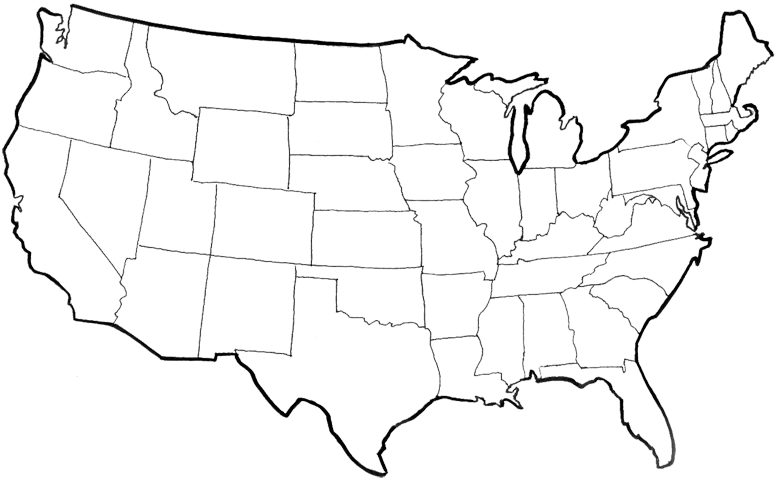
\includegraphics[width=\textwidth]{images/USA-Map-Transparent-Free-PNG-Clip-Art.png}};
    % Vertices
        \node[vertex] (S) at (-7,4.5) {S};
        \node[vertex] (L) at (-6,-2) {L};
        \node[vertex] (SF) at (-8,0.75) {SF};
        \node[vertex] (C) at (2.8,1.5) {C};
        \node[vertex] (R) at (6,-0.5) {R};
        \node[vertex] (B) at (7.5,2.9) {B};
        \coordinate (Bu) at (5.25,2.25);
    % Edges
        \path (S) edge node[above] {2043\, mi} (C) 
            edge[bend angle=15, bend right] node[below]{808\, mi}  (SF);
        \path (L)  edge node[above]{2543\, mi}  (R);
        \path (SF) edge[bend angle=15, bend right] node[above] {381\, mi} (L) 
            edge[bend angle=10, bend left] node[above]{2127\, mi}  (C);
        \path (C) edge[out=-4,in=-100] (Bu.center)
            edge node[above] {807\, mi} (R)
            edge[bend angle=10,bend right] node[above] {2015\, mi} (L);
        \path (Bu.center) edge node[pos=0,anchor=north west]{983\, mi} (B);
        \path (B) edge[bend angle=10,bend right,pos=0.6] node[above] {717\, mi} (R);
    % Helper Grid
        % \draw[gray,thin] (-8,-5) grid (8,5);
        % \draw[gray,thin,dashed,step=0.5] (-8,-5) grid (8,5);
        % \foreach \i in {-5,...,5}{
        %     \node[red,fill=white] at (0,\i) {\i};
        %     \node[red,fill=white] at (\i,0) {\i};
        % };
    \end{tikzpicture}
\end{center}
\end{practice}
